\documentclass[border=5mm]{standalone}
\usepackage{tikz}
\usepackage{fontspec} 

\begin{document}
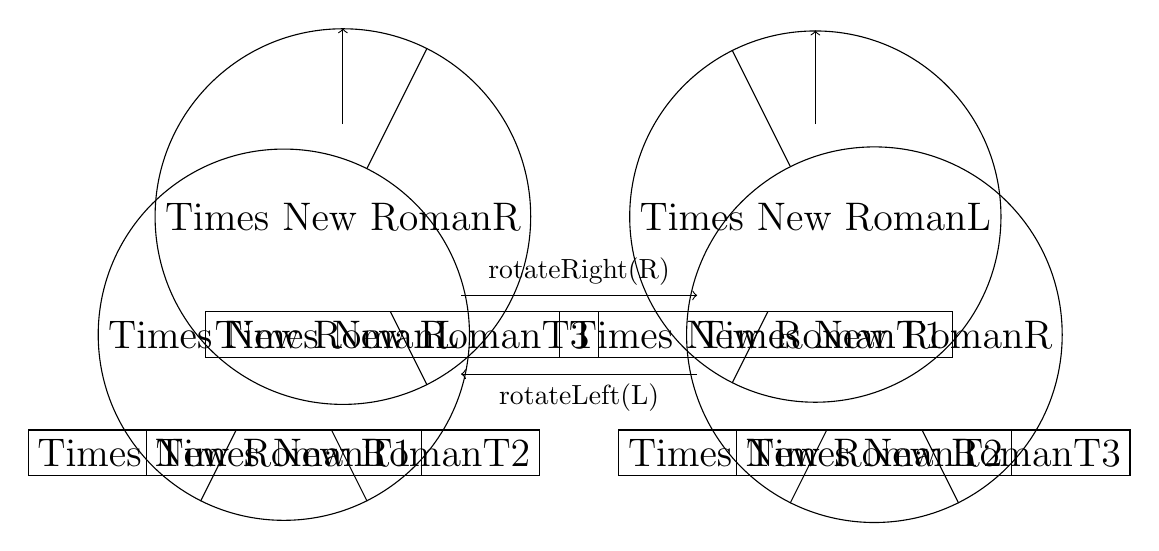
\begin{tikzpicture}

        \tikzstyle{nodebase}=[align=center, text centered, draw, font=\Large\fontspec{Times New Roman}]
        \tikzstyle{node_a}=[nodebase, circle]
        \tikzstyle{subtree}=[nodebase, rectangle]

        \node [circle] (p1) at (-3, 1) {};
        \node [node_a] (root1) at (-3,0) {R}
        child {node [node_a] {L}
                        child {node [subtree] {T1}}
                        child {node [subtree] {T2}}}
        child {node [subtree] {T3}};

        \node [circle] (p2) at (3, 1) {};
        \node [node_a] (root2) at (3,0) {L}
        child {node [subtree] {T1}}
        child {node [node_a] {R}
                        child {node [subtree] {T2}}
                        child {node [subtree] {T3}}};

        \draw[->] (p1) -- (root1);
        \draw[->] (p2) -- (root2);

        \draw[->] (-1.5,-1) -- ++(3,0) node[midway, above] {rotateRight(R)};
        \draw[->] (1.5,-2) -- ++(-3,0) node[midway, below] {rotateLeft(L)};

\end{tikzpicture}
\end{document}
